\documentclass[t]{beamer}

\usetheme{Madrid}
\usecolortheme{default}

\usepackage[utf8]{inputenc}
\usepackage{amsmath}
\usepackage{amssymb}
\usepackage{listings}
\usepackage{xcolor}
\usepackage{graphicx}
\usepackage{fancybox}
\usepackage{tikz}
\usepackage{enumerate}
\newcommand{\llbracket}{\mathopen{[\![}}
\newcommand{\rrbracket}{\mathclose{]\!]}}
\newcommand{\enc}[1]{\llbracket #1 \rrbracket}

\lstset{
  basicstyle=\ttfamily\small,
  keywordstyle=\color{blue},
  commentstyle=\color{gray},
  stringstyle=\color{red},
  breaklines=true,
  showstringspaces=false,
  tabsize=2,
  language=[Objective]Caml,
  morekeywords={let, rec, match, with, type, for, do, if, then, else, function, open}
}

\title{Value-Passing to Pure CCS Transpiler}
\subtitle{Languages for concurrency and distribution project}
\author{Jacopo Angeli  2130757}
\institute[UniPd]{Università degli studi di Padova}
\date{March 2026}

\begin{document}

\begin{frame}
\titlepage
\end{frame}

\begin{frame}[c]
  \frametitle{Outline}
  \begin{enumerate}
    \item Encoding
    \begin{enumerate}
      \item Overview
      \item Encoding Rules
    \end{enumerate}
    \item Correctness
    \begin{enumerate}
      \item Soundness of the Encoding \quad \textit{[exercise]}
    \end{enumerate}
    \item Implementation
    \begin{enumerate}
      \item AST Types
      \item Compiler
      \item Input Language
      \item Program
    \end{enumerate}
    \item Demo \& Limitations
  \end{enumerate}
\end{frame}

\section{Encoding}

  % ─── 1.1 Overview ────────────────────────────────────────────────────────────
  % Establish what the project does before diving into architecture.
  % Pipeline on the left, key points on the right.
  \begin{frame}[c]
    \frametitle{Overview}

    \begin{columns}[c]

      \column{0.3\textwidth}
      \centering
      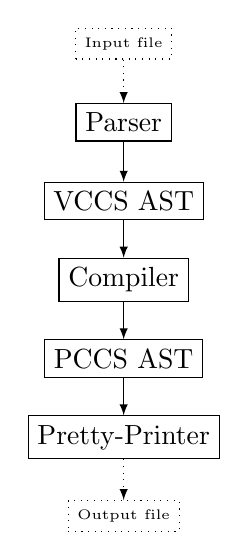
\begin{tikzpicture}[node distance=1cm, auto]
        \node (Input) [draw, dotted, rectangle] {\tiny Input file};
        \node (Parser) [draw, rectangle, align=center, below of=Input] {Parser};
        \node (VccsAST) [draw, rectangle, below of=Parser] {VCCS AST};
        \node (Compiler) [draw, rectangle, below of=VccsAST] {Compiler};
        \node (PccsAST) [draw, rectangle, below of=Compiler] {PCCS AST};
        \node (Printer) [draw, rectangle, below of=PccsAST] {Pretty-Printer};
        \node (Output) [draw, dotted, rectangle, below of=Printer] {\tiny Output file};

        \draw [dotted, -latex] (Input) -- (Parser);
        \draw [-latex] (Parser) -- (VccsAST);
        \draw [-latex] (VccsAST) -- (Compiler);
        \draw [-latex] (Compiler) -- (PccsAST);
        \draw [-latex] (PccsAST) -- (Printer);
        \draw [dotted, -latex] (Printer) -- (Output);
      \end{tikzpicture}

      \column{0.7\textwidth}
      \begin{itemize}
        \item Implements the encoding $\enc{\cdot} : \text{VCCS} \to \text{PCCS}$ from lecture
        \item Input: value-passing CCS with \textbf{interval-typed} parameters
        \item Parser: built with FsYacc/FsLex
        \item Compiler: structural recursion on the VCCS AST
        \item Output: grounded Pure Synchronisation CCS
      \end{itemize}

    \end{columns}

  \end{frame}

  % ─── 1.2 Encoding Rules ──────────────────────────────────────────────────────
  % Formal definition of [[·]] with finite interval types throughout.
  % This is the project's encoding, not the lecture's infinite version.
  \begin{frame}
    \frametitle{Encoding Rules}

    $\enc{\cdot} : \text{VCCS} \to \text{PCCS}$ \quad — all variables must be \textbf{closed} (bound before use).

    \vspace{0.2cm}

    \begin{tabular}{ll}
      $\enc{a(x{:}[L,H]).\,P}$
        &$= \displaystyle\sum_{m=L}^{H}\; a_m \,.\, \enc{P\{^m/_x\}}$ \\[8pt]
      $\enc{\overline{a}(e).\,P}$
        &$= \overline{a}_m \,.\, \enc{P}$ \quad ($e \!\downarrow\! m$) \\[4pt]
      $\enc{\tau.\,P}$
        &$= \tau \,.\, \enc{P}$ \\[4pt]
      $\enc{P \mid Q}$
        &$= \enc{P} \mid \enc{Q}$ \\[4pt]
      $\enc{P \setminus \{c{:}[L,H]\}}$
        &$= \enc{P} \setminus \{\,c_L,\; c_{L+1},\; \ldots,\; c_H\,\}$ \\[4pt]
      $\enc{P\;[\,a / b {:} [L,H]\,]}$
        &$= \enc{P}[f']$ \quad $f'(a_m)=b_m,\;\; f'(\overline{a}_m)=\overline{b}_m \quad m \in [L,H]$ \\[4pt]
      $\enc{\text{if } b \text{ then } P \text{ else } Q}$
        &$= \begin{cases} \enc{P} & b \text{ true} \\ \enc{Q} & b \text{ false}\end{cases}$ \\[8pt]
      $\enc{K(e_1,\ldots,e_h)}$
        &$= K_{n_1,\ldots,n_h}$ \quad ($e_i \!\downarrow\! n_i$) \\[4pt]
    \end{tabular}

    \vspace{0.15cm}
    \small $K_{n_1,\ldots,n_h} \;\overset{\text{def}}{=}\; \enc{P\{^{n_1}/_{x_1},\ldots,^{n_h}/_{x_h}\}}$
    \quad where $K(x_1{:}[L_1,H_1],\ldots,x_h{:}[L_h,H_h]) \overset{\text{def}}{=} P$ and $n_i \in [L_i, H_i]$

  \end{frame}

\section{Correctness}

  % ─── 2. Correctness theorem (both parts) ──────────────────────────────────────
  % Exact theorem statement from lecture (10/03, page 7): proof is the exam exercise.
  % Part (i) soundness + part (ii) completeness. Proof sketch for both.
  \begin{frame}
    \frametitle{Correctness of the Encoding \quad \textit{[exam exercise]}}

    \begin{alertblock}{Theorem (lecture, 10/03)}
      For all programs $P$ in CCS-VP, where
      $\hat{\alpha} = a_m$ if $\alpha = a(m)$,\; $\overline{a}_m$ if $\alpha = \overline{a}(m)$,\; $\tau$ if $\alpha = \tau$:
      \begin{enumerate}[(i)]
        \item \textbf{Soundness:}\quad $P \xrightarrow{\alpha} P'
              \;\Longrightarrow\; \enc{P} \xrightarrow{\hat{\alpha}} \enc{P'}$
        \item \textbf{Completeness:}\quad $\enc{P} \xrightarrow{\hat{\alpha}} Q
              \;\Longrightarrow\; \exists P'.\; P \xrightarrow{\alpha} P' \text{ and } \enc{P'} = Q$
      \end{enumerate}
    \end{alertblock}

    \vspace{0.2cm}

    \textbf{Proof of (i)} by induction on the derivation of $P \xrightarrow{\alpha} P'$:
    \begin{itemize}
      \item \textbf{Input:} $a(x).P \xrightarrow{a(m)} P\{^m/_x\}$.
            $\enc{a(x).P} = \sum_m a_m.\enc{P\{^m/_x\}}$;\;
            branch $a_m$ fires. \checkmark
      \item \textbf{Output:} $\overline{a}(e).P \xrightarrow{\overline{a}(m)} P$, $e \!\downarrow\! m$.
            $\enc{\overline{a}(e).P} = \overline{a}_m.\enc{P}$;\; fires on $\overline{a}_m$. \checkmark
      \item \textbf{$\tau$, Sum, Par, Res, Rel, Const:} immediate by IH + corresponding PCCS rules.
    \end{itemize}

    \vspace{0.1cm}
    \textbf{Proof of (ii)} by induction on the derivation of $\enc{P} \xrightarrow{\hat{\alpha}} Q$:
    each PCCS branch $a_m$ in $\enc{a(x).P}$ corresponds to exactly one VCCS transition
    $a(x).P \xrightarrow{a(m)} P\{^m/_x\}$, so the witness $P'$ is recovered uniquely.

  \end{frame}

\section{Implementation}

  % ─── 3.1 AST Types ───────────────────────────────────────────────────────────
  % Show Vccs.P vs Pccs.P side by side.
  % Key difference: Vccs carries typed variables and AExp; Pccs has only plain strings.
  % No Conditional in PCCS: guards are resolved at compile time.
  \begin{frame}[fragile]
    \frametitle{AST Types}

    \begin{columns}[t]
      \column{0.5\textwidth}
      \textbf{Vccs.P} \quad (value-carrying)
      \begin{lstlisting}[basicstyle=\ttfamily\scriptsize]
type Action =
  | Input  of string
           * (string * Interval)
  | Output of string * AExp
  | Silent

type P =
  | Act         of Action * P
  | Conditional of BExp * P * P
  | Sum         of P * P
  | Parallel    of P * P
  | Restrict    of P * (string * Interval) list
  | Rename      of P
               * (string * string * Interval) list
  | ConstCall   of string * AExp list
  | Nil
      \end{lstlisting}

      \column{0.5\textwidth}
      \textbf{Pccs.P} \quad (ground names)
      \begin{lstlisting}[basicstyle=\ttfamily\scriptsize]
type Action =
  | Input  of string  (* "a_3"   *)
  | Output of string  (* "a_3"   *)
  | Silent

type P =
  | Act       of Action * P
  (* no Conditional: resolved *)
  | Sum       of P * P
  | Parallel  of P * P
  | Restrict  of P * string list
  | ConstCall of string (* "Q_2_1" *)
  | Nil
      \end{lstlisting}
    \end{columns}

    \vspace{0.2cm}
    \small
    \texttt{Conditional} and \texttt{AExp} disappear: guards are evaluated
    and branches selected at compile time under a concrete environment.

  \end{frame}

  % ─── 3.2 Compiler ────────────────────────────────────────────────────────────
  % compileP: structural recursion, environment threading.
  % getValuations: cartesian product of parameter domains.
  % Show the three key cases (Input, Output, Conditional) + parameterised constants.
  \begin{frame}[fragile]
    \frametitle{Compiler}

    \begin{columns}[t]
      \column{0.57\textwidth}
      \begin{lstlisting}[basicstyle=\ttfamily\scriptsize]
let rec compileP (P: Vccs.P)
                 (env: (string*int) list)
               : Pccs.P =
  match P with
  | Act(Input(ch,(x,ty)), P) ->
      Interval.toList ty
      |> List.map (fun v ->
          Pccs.Act(
            Input(sprintf "%s_%d" ch v),
            compileP P ((x,v)::env)))
      |> List.reduce Pccs.Sum

  | Act(Output(ch,e), P) ->
      Pccs.Act(
        Output(sprintf "%s_%d" ch (eval e env)),
        compileP P env)

  | Conditional(b, p, q) ->
      if evalB b env
      then compileP p env
      else compileP q env

  | ConstCall(K, args) ->
      let vs = List.map (eval env) args
      Pccs.ConstCall(K + joinWith "_" vs)
  ...
      \end{lstlisting}

      \column{0.43\textwidth}
      \vspace{0.3cm}
      \begin{itemize}
        \item \texttt{env} maps variable names to their current concrete integer values
        \item For parameterised declarations: \texttt{getValuations} computes the cartesian product of all domains, one compiled definition per valuation
        \item \texttt{ConstCall} arguments are evaluated and embedded in the name
        \item \texttt{Rename}: each \texttt{(fromCh, toCh, [L,H])} generates pairs $a_m \to b_m$ for \emph{both} input and output directions, for all $m \in [L,H]$ — directly implements $f'(a_m) = f(a)_m$
      \end{itemize}

    \end{columns}

  \end{frame}

  % ─── 3.3 Input Language ──────────────────────────────────────────────────────
  % VCCS concrete syntax: what the user writes in a .vccs file.
  % Two-column layout: left = syntax cheat-sheet, right = worked example.
  \begin{frame}[fragile]
    \frametitle{Input Language}

    Built with \textbf{FsLexYacc}: \texttt{.fsl} + \texttt{.fsy} $\rightarrow$ F\# lexer and parser modules.

    \vspace{0.2cm}

    \begin{columns}[t]
      \column{0.52\textwidth}
      \textbf{Syntax}
      \begin{lstlisting}[basicstyle=\ttfamily\scriptsize]
(* declaration *)
P = proc
P(x:[0,5], y:[0,2]) = proc

(* process *)
'a(e).P         (* output *)
a(x:[0,5]).P    (* input *)
tau.P
P + P           (* choice *)
P | P           (* parallel *)
P \ {c:[0,5]}   (* restriction *)
P [a / b : [0,5]] (* renaming *)
if b then P else P
K(e1, e2)  |  nil
      \end{lstlisting}

      \column{0.48\textwidth}
      \textbf{Example}
      \begin{lstlisting}[basicstyle=\ttfamily\scriptsize]
P = a(x:[0,2]).Q(x);

Q(x:[0,1]) =
  if x != 0
  then tau.Q(x)
  else 'done(0).nil;
      \end{lstlisting}

      \vspace{0.3cm}
      \small Expressions \texttt{e}: \texttt{+}, \texttt{-}, \texttt{*}, \texttt{/}\\
      Guards \texttt{b}: \texttt{==}, \texttt{!=}, \texttt{<}, \texttt{>}, \texttt{\&\&}, \texttt{||}

    \end{columns}

  \end{frame}

  % ─── 3.4 Program ─────────────────────────────────────────────────────────────
  % Two modes: file mode and interactive REPL.
  % REPL supports multi-line input (terminated by ';') and #list / #clear / #quit.
  \begin{frame}[fragile]
    \frametitle{Program}

    Two execution modes:

    \vspace{0.3cm}

    \textbf{File mode}
    \begin{lstlisting}[language={}, basicstyle=\ttfamily\scriptsize]
$ dotnet run --project V2Pccs.fsproj input.vccs
  Parsed successfully.
  Compiled successfully.
Output written to: input.ccs
    \end{lstlisting}

    \vspace{0.3cm}

    \textbf{Interactive REPL}
    \begin{lstlisting}[language={}, basicstyle=\ttfamily\scriptsize]
$ dotnet run --project V2Pccs.fsproj
vccs> B = in(x:[0,1]).'out(x).B;
B = (in_0.'out_0.B + in_1.'out_1.B)
vccs> #list
  B
vccs> #quit
    \end{lstlisting}

    \vspace{0.2cm}
    \small Undefined-reference warnings are emitted after each compilation unit.

  \end{frame}

\section{Demo \& Limitations}

  % ─── 4.1 Demo ─────────────────────────────────────────────────────────────────
  % Show the lecture Buffer example compiled, then go live.
  \begin{frame}[fragile]
    \frametitle{Demo}

    \textbf{Worked example} — lecture Buffer:

    \vspace{0.2cm}

    \begin{columns}[t]
      \column{0.45\textwidth}
      \textbf{Input} (\texttt{.vccs})
      \begin{lstlisting}[basicstyle=\ttfamily\scriptsize]
B  = in(x:[0,2]).'out(x).B;
B' = 'in(0).B';
      \end{lstlisting}

      \column{0.55\textwidth}
      \textbf{Output} (\texttt{.ccs})
      \begin{lstlisting}[basicstyle=\ttfamily\scriptsize]
B = (in_0.'out_0.B
   + in_1.'out_1.B
   + in_2.'out_2.B)
B' = 'in_0.B'
      \end{lstlisting}
    \end{columns}

    \vspace{0.4cm}
    \textit{Live demo follows.}

  \end{frame}

  % ─── 4.2 Limitations ─────────────────────────────────────────────────────────
  % Pick the four most important known limitations.
  \begin{frame}
    \frametitle{Limitations}

    \begin{enumerate}

      \item \textbf{Interval types only} \\
            Enumeration types from the spec (e.g.\ $\{a, b, c\}$) are not supported.

      \vspace{0.2cm}

      \item \textbf{Domain explosion} \\
            $n$ parameters each with domain size $d$ generate $d^n$ definitions.
            No dead-code elimination or deduplication.

      \vspace{0.2cm}

      \item \textbf{No static type checking} \\
            Undefined constant references surface only as post-compilation
            warnings, not as errors before code generation.

    \end{enumerate}

  \end{frame}

\end{document}
